\clearpage
\makeatletter
\efloat@restorefloats
\makeatother


\begin{appendix}
\section{}
\setlength{\parindent}{0.0in}
\setlength{\leftskip}{0.0in}

\hypertarget{appendix-1-the-mathematical-development-of-the-f-test-w-test-and-f-test-numerical-example}{%
\subsection{\texorpdfstring{Appendix 1: The Mathematical Development of
the \emph{F}-test, \emph{W}-test, and \emph{F}*-test: Numerical
Example}{Appendix 1: The Mathematical Development of the F-test, W-test, and F*-test: Numerical Example}}\label{appendix-1-the-mathematical-development-of-the-f-test-w-test-and-f-test-numerical-example}}

A summary is presented in Table A1. The complete example is available on
Github. The DV is a score that can vary from 0 to 40. The IV is a
three-level factor A (levels = \(A_1\), \(A_2\) and \(A_3\)).

\begin{figure}
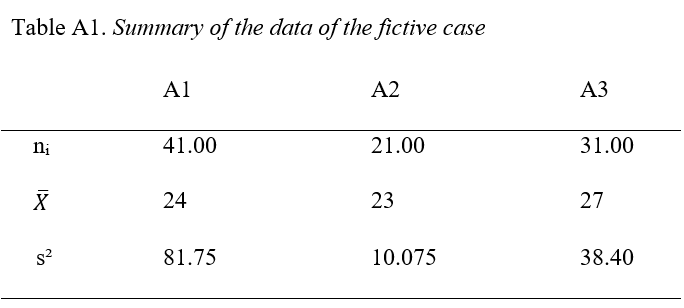
\includegraphics[width=1\linewidth]{Rmarkdown folder/Rmarkdown inputs/TableA1} \end{figure}

The global mean (i.e.~the mean of the global dataset) is a weighted mean
of the group means:

\[\frac{(41*24)+(21*23)+(31*27)}{41+21+31}=\frac{2304}{93} \approx 24.77\]

The \emph{F}-test statistic and degrees of freedom are computed by
applying formulas (1), (2) and (3):

\[
F=\frac{\frac{1}{3-1}[41*(24-\frac{2304}{93})^2+21*(23-\frac{2304}{93})^2+31*(27-\frac{2304}{93})^2]}
{\frac{1}{93-3}[(41-1)*81.75+(21-1)*10.07+(31-1)*38.40]} \approx 2.38
\]

\[
df_n=3-1=2
\]

\[
df_d=93-3=90
\]

The \emph{F}*-test and his degrees of freedom are computed by applying
formulas 4, 5 and 6:

\[
F^*=\frac{41*(24-\frac{2304}{93})^2+21*(23-\frac{2304}{93})^2+31*(27-\frac{2304}{93})^2}{(1-\frac{41}{93})*81.75+(1-\frac{21}{93})*10.07+(1-\frac{31}{93})*38.40} \approx 3.09
\]

\[
df_n=3-1=2
\]

\[
df_d=\frac{1}{\frac{(\frac{(1-\frac{41}{93})*81.75}{\sum_{j=1}^k(1-\frac{n_j}{N})s_j^2})^2}{41-1}+\frac{(\frac{(1-\frac{21}{93})*10.07}{\sum_{j=1}^k(1-\frac{n_j}{N})s_j^2})^2}{21-1}+\frac{(\frac{(1-\frac{31}{93})*38.40}{\sum_{j=1}^k(1-\frac{n_j}{N})s_j^2})^2}{31-1}} \approx 81.15
\]

\[ Where \sum_{j=1}^k(1-\frac{n_j}{N})*s_j^2 \approx 79.11\]

Finally, the \emph{W}-test and his degrees of freedom are computed in
applying formulas 7, 8 and 9:

\[
W=\frac{\frac{1}{3-1}[\frac{41}{81.75}(24-\bar{X'})^2+\frac{21}{10.07}(23-\bar{X'})^2+\frac{31}{38.40}(27-\bar{X'})^2]}
{\frac{2(3-2)}{3^2-1}[(\frac{1}{41-1})(1-\frac{\frac{41}{81.75}}{w})^2+(\frac{1}{21-1})(1-\frac{\frac{21}{10.07}}{w})^2+(\frac{1}{31-1})(1-\frac{\frac{31}{38.40}}{w})^2]+1} \approx 4.61
\]

Where:

\(w=\sum_{j=1}^k w_j \approx 3.39\)

\(\bar{X'}=\frac{\sum_{j=1}^k (w_j\bar{x_j})}{w} \approx 24.10\)

\[
df_n=3-1
\]

\[
df_d=\frac{3^2-1}{3[\frac{(1-\frac{w_j}{w})^2}{41-1}+\frac{(1-\frac{w_j}{w})^2}{21-1}+\frac{(1-\frac{w_j}{w})^2}{31-1}]} \approx 59.32
\]

One should notice that in this example, the biggest sample size has the
biggest variance. As previously mentioned, it means that the
\emph{F}-test will be too conservative, because the \emph{F} value
decreases. The \emph{F}*-test will also be a little too conservative,
even if the test is less affected than the \emph{F}-test. As a
consequence: \emph{W} \textgreater{} \emph{F}* \textgreater{} \emph{F}.

\hypertarget{appendix-2-justification-for-the-choice-of-distributions-in-simulations}{%
\subsection{Appendix 2: Justification for the choice of distributions in
simulations}\label{appendix-2-justification-for-the-choice-of-distributions-in-simulations}}

The set of simulations described in the article was repeated for 7
distributions. We used R commands to generate data from different
distributions:

\begin{itemize}
\item
  \emph{k} normal distributions (Figure A1): in order to assess the Type
  I error rate and power of the different tests under the assumption of
  normality, data were generated by means of the function ``rnorm''
  (from the package ``stats''; ``R: The Normal Distribution,'' 2016).
\item
  \emph{k} double exponential distributions (Figure A2): In order to
  assess the impact of high kurtosis on the Type I error rate and power
  of all tests, data were generated by means of the function
  ``rdoublex'' (from the package ``smoothmest''; ``R: The double
  exponential (Laplace) distribution,'' 2012).
\item
  \emph{k} mixed normal distributions (Figure A3): In order to assess
  the impact of extremely high kurtosis on the Type I error rate and
  power of all tests, regardless of variance, data were generated by
  means of the function ``rmixnorm'' (from the package ``bda''; Wang \&
  Wang, 2015).
\item
  \emph{k} normal right skewed distributions (Figure A4): In order to
  assess the impact of moderate skewness on the Type I error rate and
  power, data were generated by means of the function ``rsnorm'' (from
  the package ``fGarch''; ``R: Skew Normal Distribution,'' 2017). The
  normal skewed distribution was chosen because it is the only skewed
  distribution where the standard deviation ratio can vary without
  having an impact on skewness.
\item
  \emph{k}-1 normal left skewed distributions (Figure A5) and 1 normal
  right skewed distribution (Figure A2.4): In order to assess the impact
  of unequal shapes, in terms of skewness, on the Type I error rate and
  power, when data have moderate skewness, data were generated by means
  of the functions ``rsnorm'' (from the package ``fGarch''; ``R: Skew
  Normal Distribution,'' 2017).
\item
  \emph{k}-1 chi-squared distributions with two degrees of freedom (See
  Figure A6), and one normal rigt skewed distribution (Figure A2.4): In
  order to assess the impact of high asymetry on the Type I error rate
  an power, k-1 distributions were generated by means of the functions
  ``rchisq'' (``R: The (non-central) Chi-squared Distribution,'' 2016).
  The last distribution was generated by means of ``rsnorm'' in order to
  follow a normal right skewed distribution with a mean of 2 (from the
  package ``fGarch''; ``R: Skew Normal Distribution,'' 2017). Because
  the chi-squared is non-negative, it is not possible to generate
  chi-squared where population SD= 1, 4 or 8 and population mean is the
  same than the chi-squared with two degrees of freedom. However, we
  wanted to assess the impact of different SD-ratio on Type I error
  rate. For these reasons, the last distribution was generated by means
  of ``rsnorm'' in order to follow a normal skewed distribution with
  positive skewness of +0.99 and mean = 2 (from the package ``fGarch'';
  ``R: Skew Normal Distribution,'' 2017).
\item
  \emph{k}-1 chi-squared distributions with two degrees of freedom (See
  Figure A6), and one normal left skewed distribution (Figure A5): In
  order to assess the impact of unequal shapes, in terms of skewness, on
  Type I error rate and power when distributions have extreme skewness,
  k-1 distributions were generated by means of the functions ``rchisq''
  (``R: The (non-central) Chi-squared Distribution,'' 2016). The last
  distribution was generated by means of ``rsnorm'' in order to follow a
  normal right skewed distribution with a mean of 2 (from the package
  ``fGarch''; ``R: Skew Normal Distribution,'' 2017)
\end{itemize}

\begin{figure}
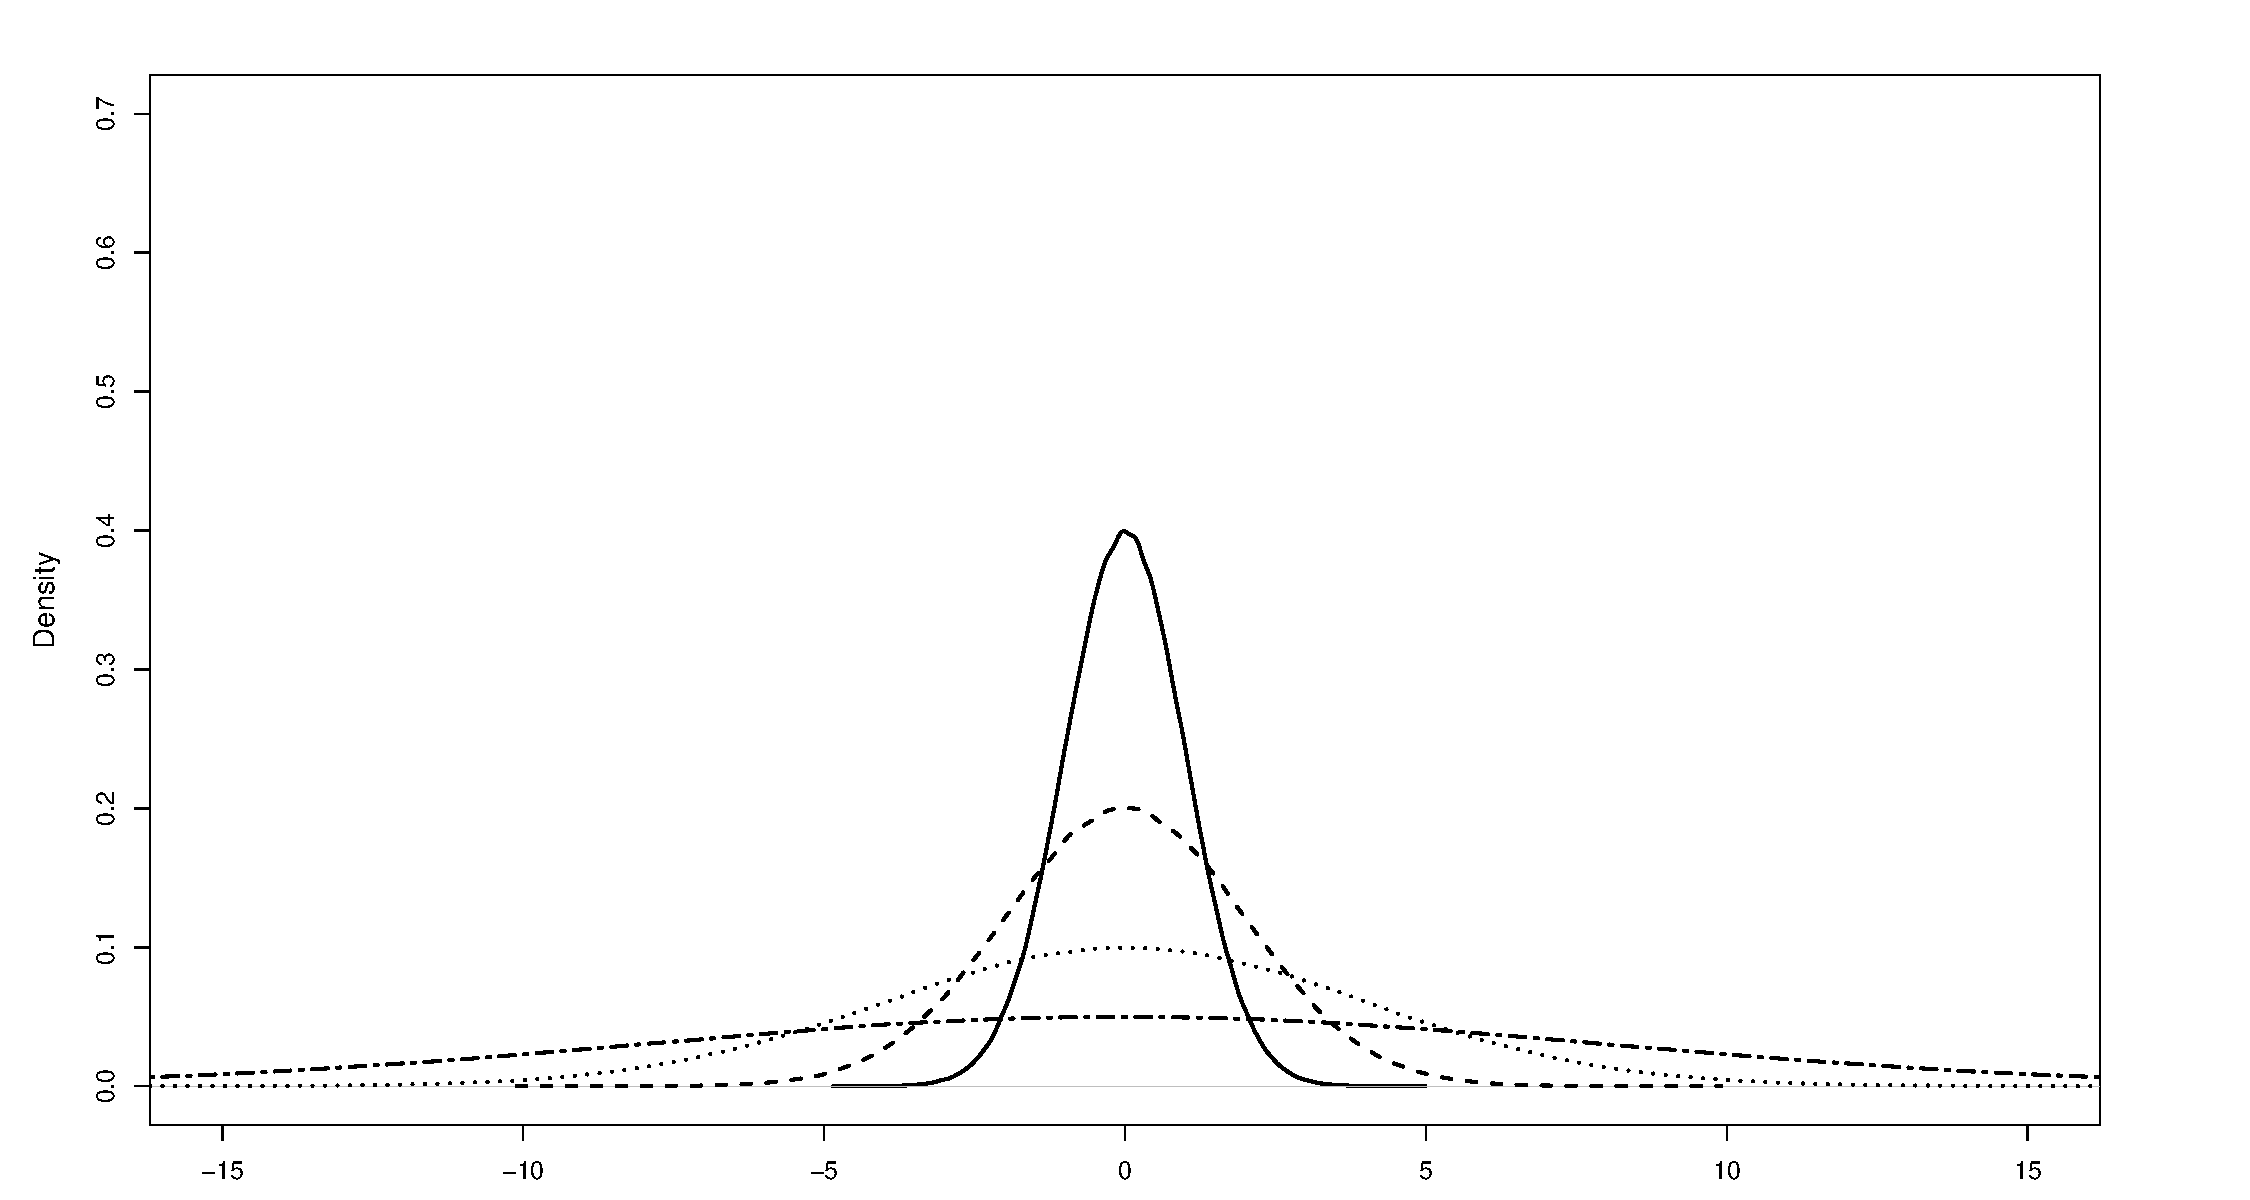
\includegraphics[width=400px]{W-test_files/figure-latex/unnamed-chunk-17-1} \caption{centered normal probability density function, as a function of the population SD}(\#fig:unnamed-chunk-17)
\end{figure}

\begin{figure}
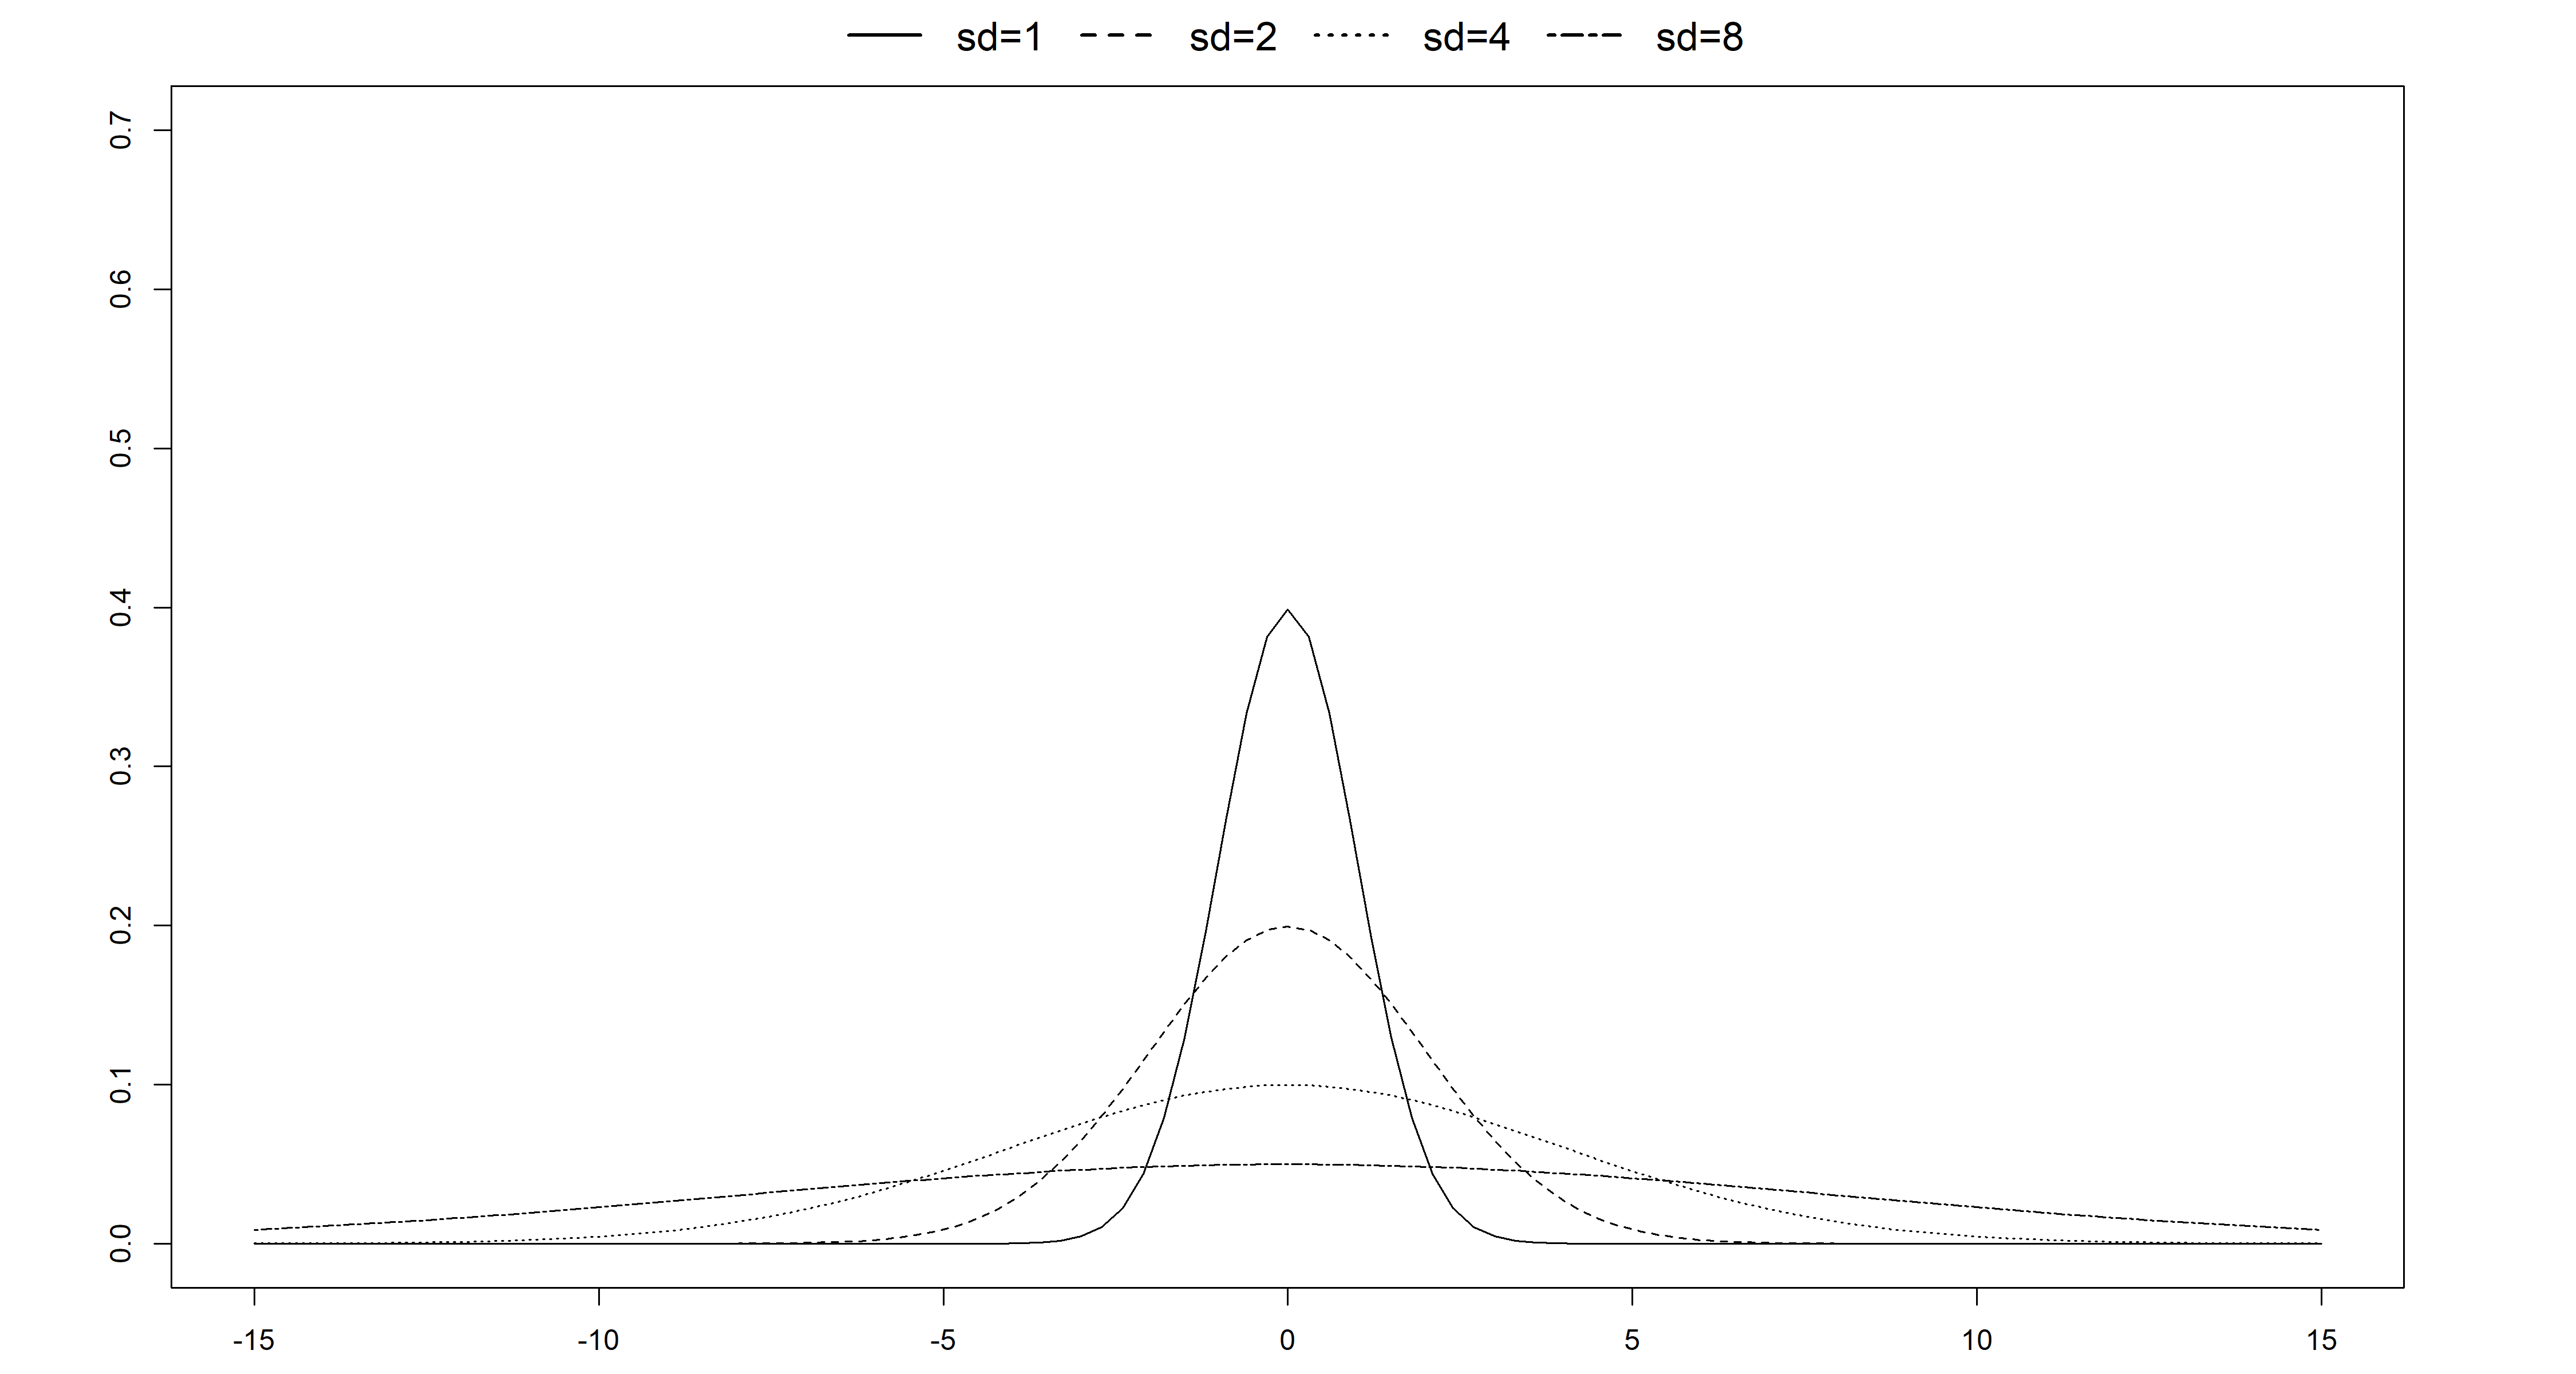
\includegraphics[width=400px]{W-test_files/figure-latex/unnamed-chunk-18-1} \caption{centered double exponential probability density function, as a function of the population SD}(\#fig:unnamed-chunk-18)
\end{figure}

\begin{figure}
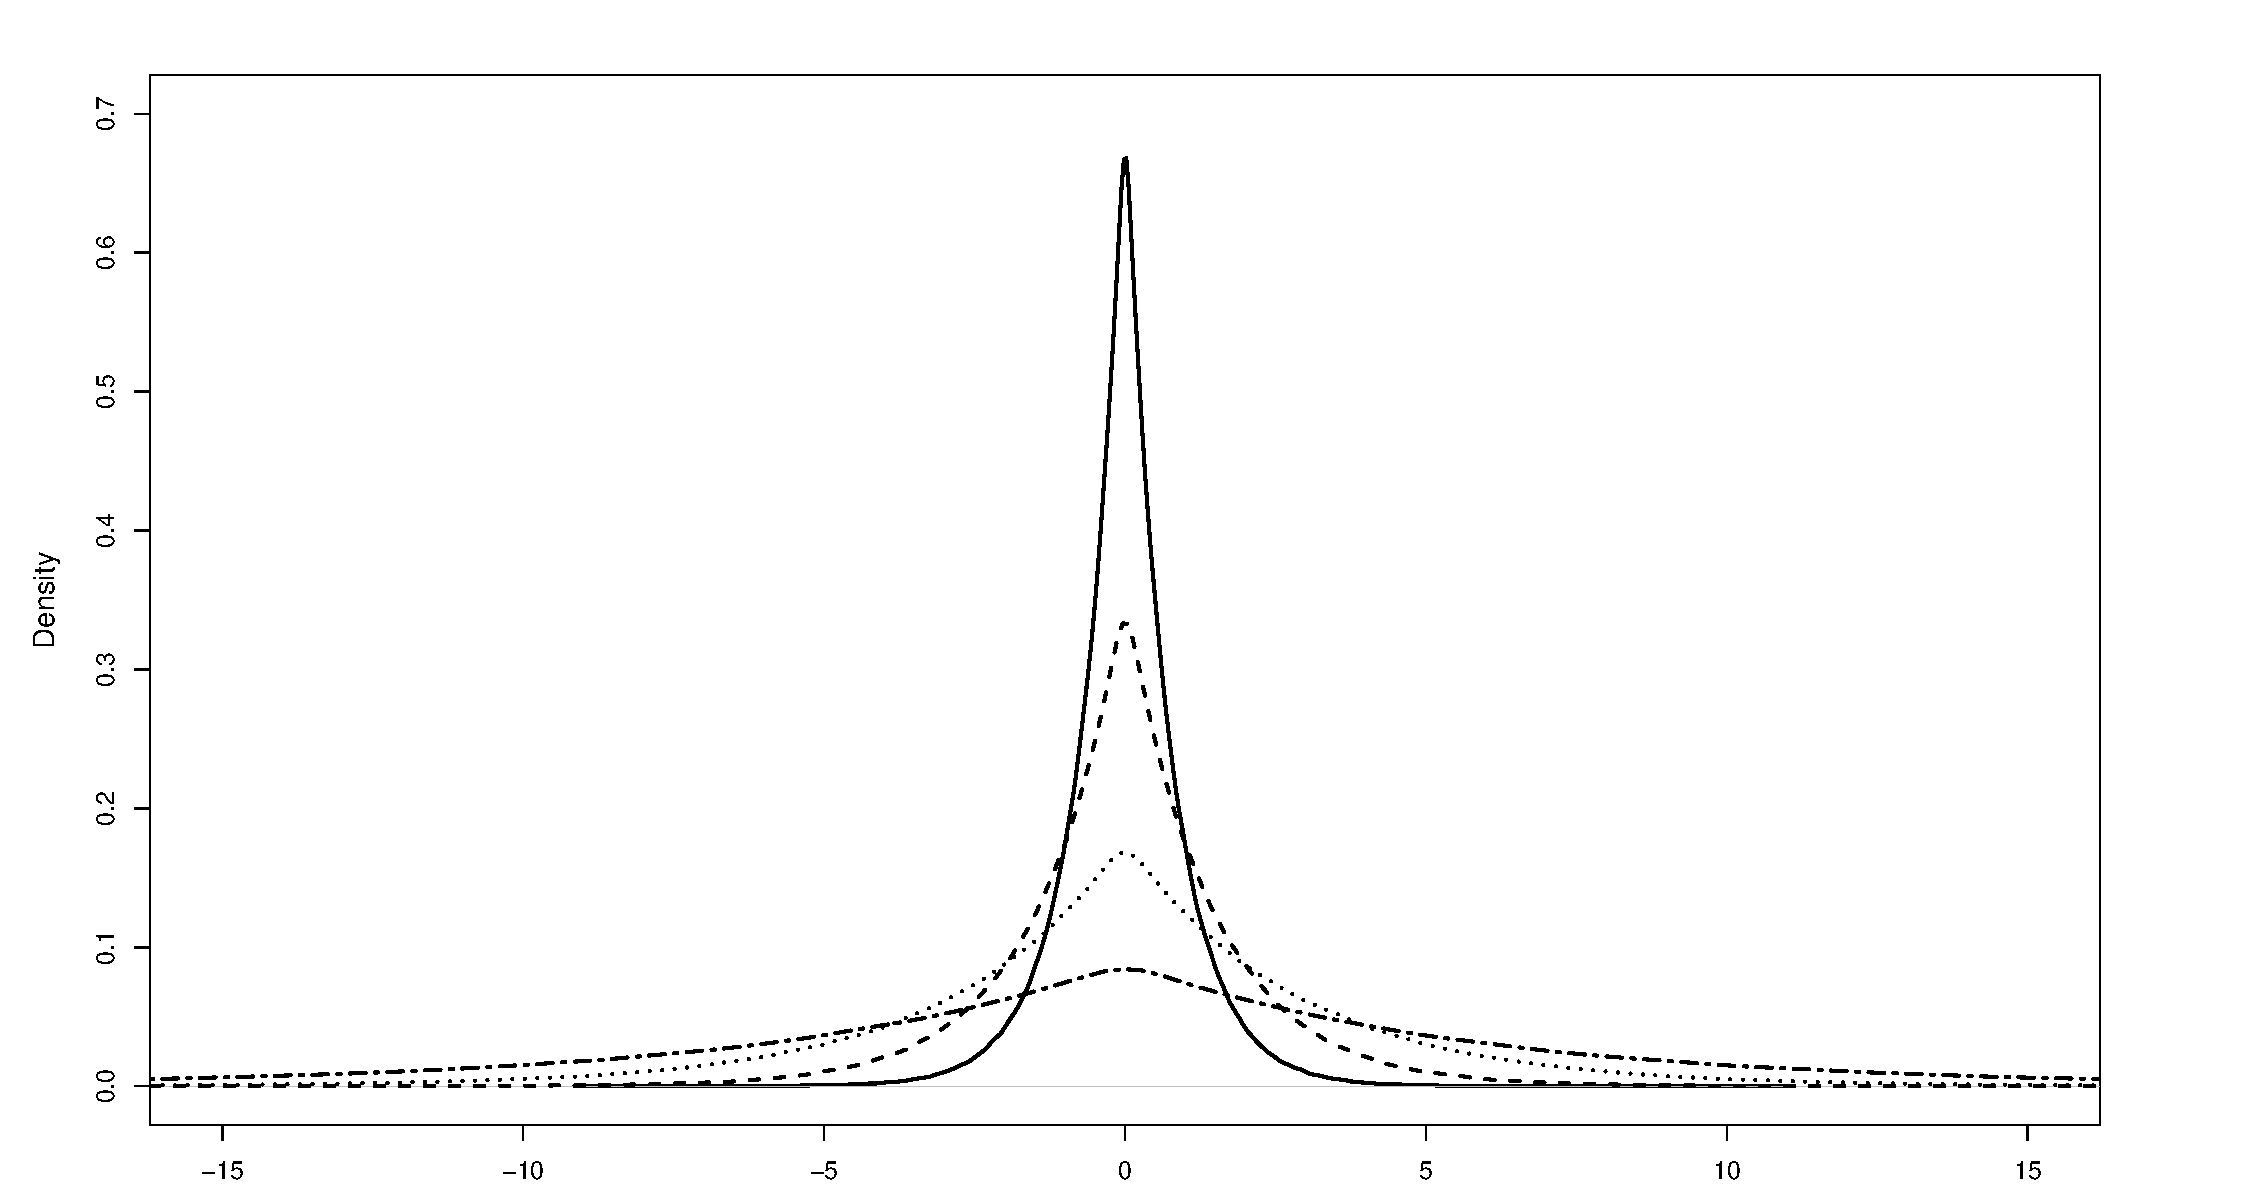
\includegraphics[width=400px]{W-test_files/figure-latex/unnamed-chunk-19-1} \caption{centered mixed normal probability density function, as a function of the population SD}(\#fig:unnamed-chunk-19)
\end{figure}

\#\texttt{\{r\ "",\ echo=FALSE,\ fig.width\ =\ 15,fig.height=8,out.width\ =\ \textquotesingle{}400px\textquotesingle{},fig.cap\ =\ "centered\ normal\ right\ \#\#skewed\ robability\ density\ function,\ as\ a\ function\ of\ the\ population\ SD"\}\ \#n=1000000\ \#NP1=rsnorm(n,\ mean=0,\ sd=1,xi=10)\ \ \#NP2=rsnorm(n,\ mean=0,\ sd=2,xi=10)\ \ \#NP3=rsnorm(n,\ mean=0,\ sd=4,xi=10)\ \ \ \#NP4=rsnorm(n,\ mean=0,\ sd=8,xi=10)\ \ \ \#par(mai=c(.5,1,.5,1))\ \#plot(density(NP1),lty=1,xlim=c(-15,15),ylim=c(0,.7),lwd=2,main="",xlab="",cex.lab=1.2)\ \#lines(density(NP2),lty=2,lwd=2)\ \#lines(density(NP3),lty=3,lwd=2)\ \#lines(density(NP4),lty=6,lwd=2)\ \#legend(0,.83,legend=c("sd=1","sd=2","sd=4","sd=8"),lty=c(1,2,3,6),lwd=c(2,2,2,2),bty="n",xjust=0.5,yjust=1,\#horiz=TRUE,xpd=TRUE,cex=1.2)\ \#}

\#\texttt{\{r\ "",\ echo=FALSE,\ fig.width\ =\ 15,fig.height=8,out.width\ =\ \textquotesingle{}400px\textquotesingle{},fig.cap\ =\ "centered\ normal\ left\ \#skewed\ probability\ density\ function,\ as\ a\ function\ of\ the\ population\ SD"\}\ \#n=1000000\ \ \#NN1=rsnorm(n,\ mean=0,\ sd=1,xi=-10)\ \ \#NN2=rsnorm(n,\ mean=0,\ sd=2,xi=-10)\ \ \#NN3=rsnorm(n,\ mean=0,\ sd=4,xi=-10)\ \ \ \#NN4=rsnorm(n,\ mean=0,\ sd=8,xi=-10)\ \ \ \#par(mai=c(.5,1,.5,1))\ \#plot(density(NN1),lty=1,xlim=c(-15,15),ylim=c(0,.7),lwd=2,main="",xlab="",cex.lab=1.2)\ \#lines(density(NN2),lty=2,lwd=2)\ \#lines(density(NN3),lty=3,lwd=2)\ \#lines(density(NN4),lty=6,lwd=2)\ \#legend(0,.83,legend=c("sd=1","sd=2","sd=4","sd=8"),lty=c(1,2,3,6),lwd=c(2,2,2,2),bty="n",xjust=0.5,yjust=1,\#horiz=TRUE,xpd=TRUE,cex=1.2)\ \#}

\begin{figure}
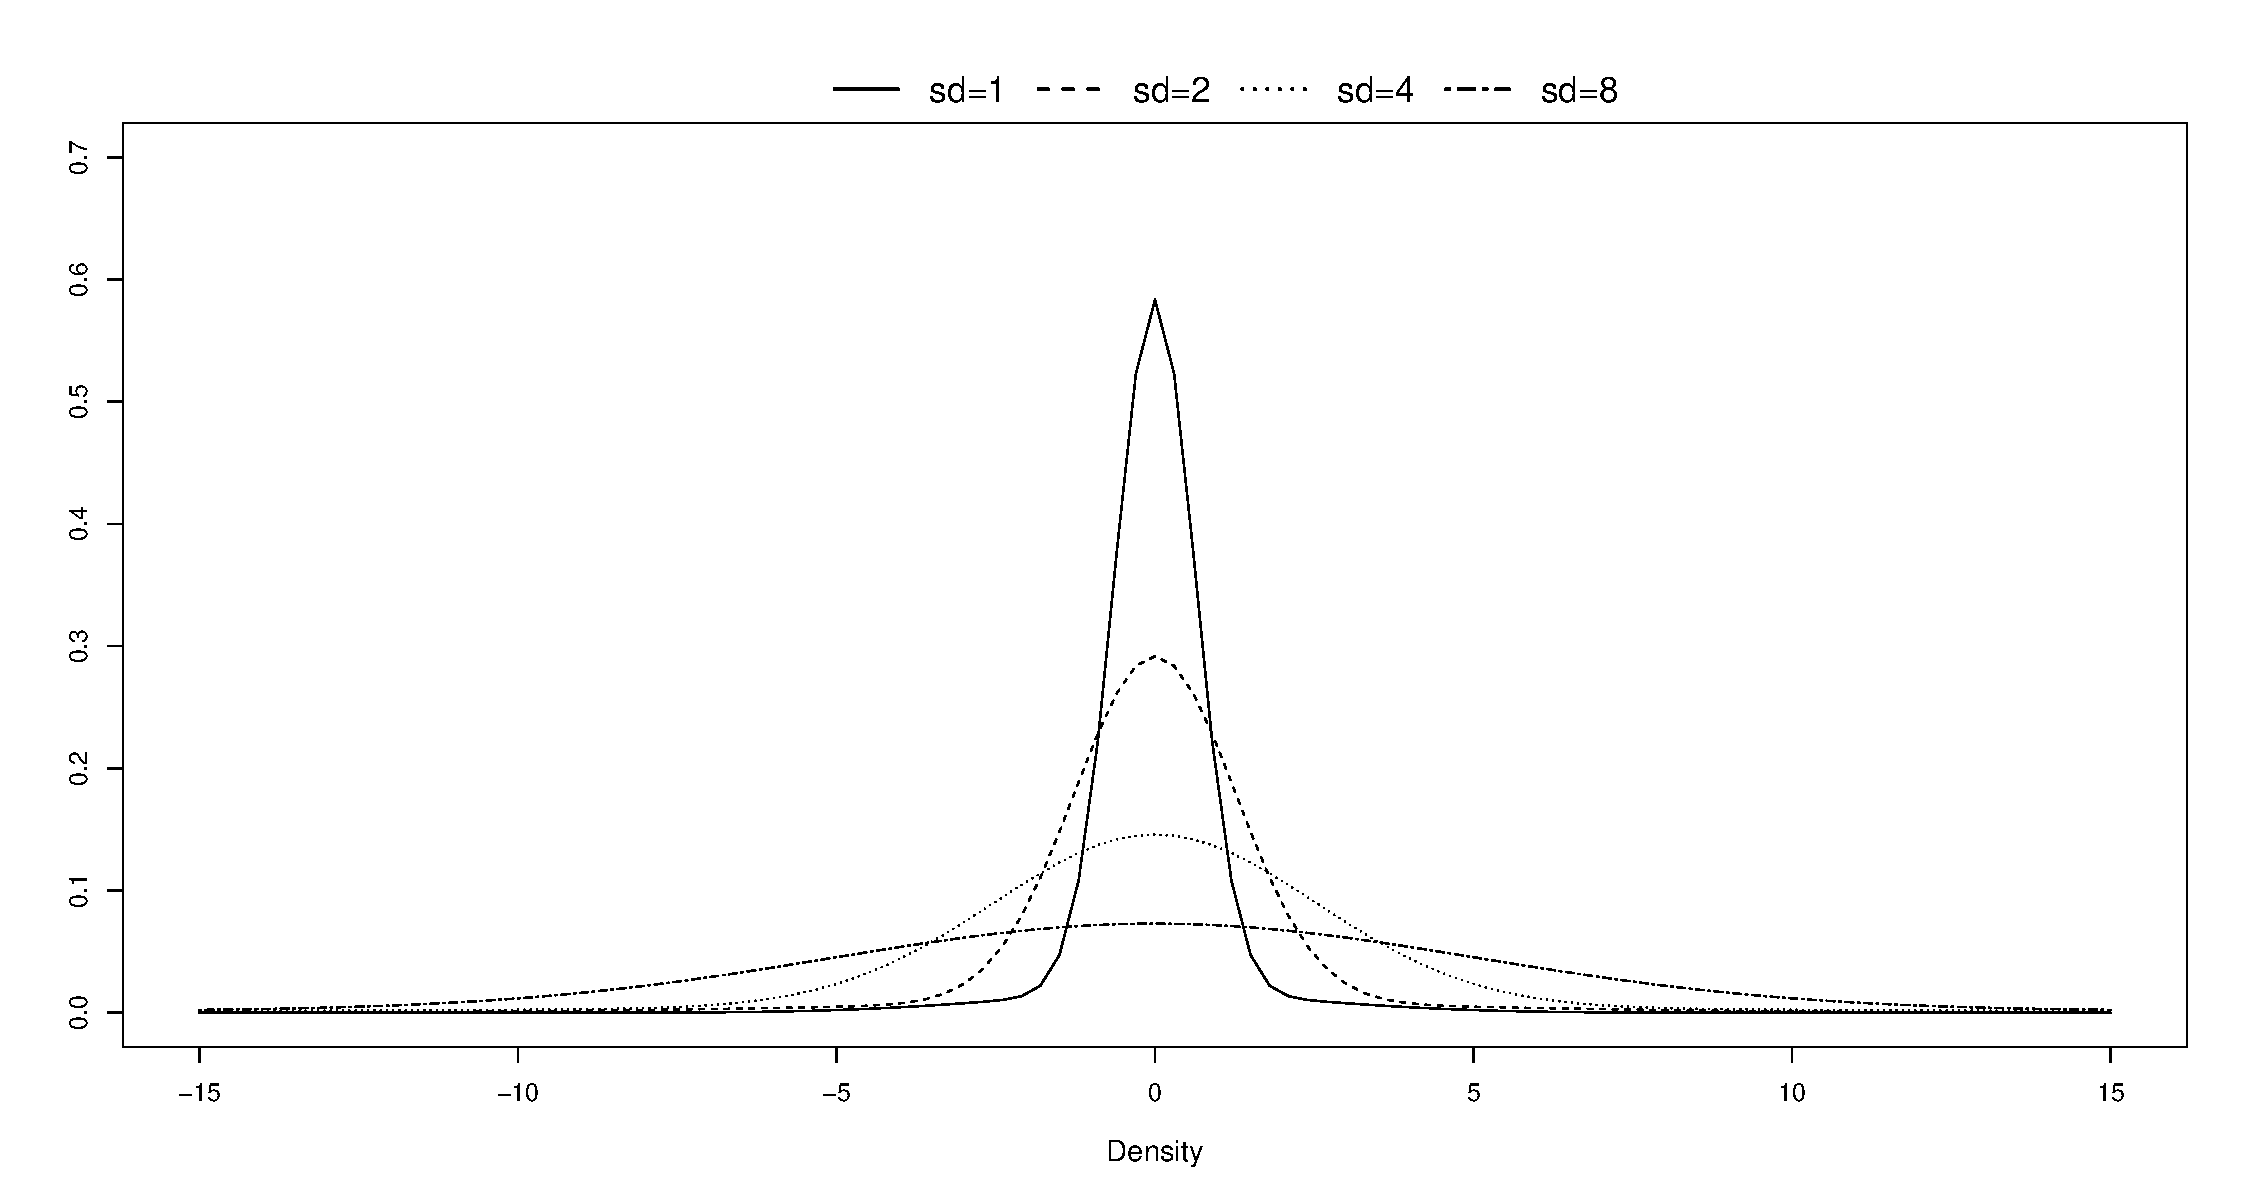
\includegraphics[width=400px]{W-test_files/figure-latex/unnamed-chunk-20-1} \caption{chi-squared with 2 degrees of freedom probability density function, as a function of the population SD}(\#fig:unnamed-chunk-20)
\end{figure}
\end{appendix}
